\lecture{2009-11-11}

\subsection{Polynom-Interpolation (Basis CAD/CAGD)}

\subsubsection*{Interpolation}
\label{interpolation}%
gegeben: Daten $(x_k, y_k)\;k=0,\ldots,n$\\
konstruiere Polynom $P(x)$: $P(x_k) = y_k$
%
\[ P(x) = a_0 + a_1x + \ldots + a_nx^n \]
\vspace{-1cm}
\begin{align*}
&a_0 + a_1x_0 + a_2x_0^2 + \ldots + a_nx_0^n = y_0 \\
&\vdots \\
&a_0 + a_1x_n + a_2x_n^2 + \ldots + a_nx_n^n = y_n
\end{align*}
\[
A = 
\begin{pmatrix}
	1 & x_0 & x_0^2 & \cdots & x_0^n \\
	1 & x_1 & x_1^2 & \cdots & x_1^n \\
	\vdots & \vdots & \vdots & \ddots & \vdots \\
	1 & x_n & x_n^2 & \cdots & x_n^n
\end{pmatrix} \quad
b = \begin{pmatrix}	y_0 \\	y_1 \\	\vdots \\	y_n \end{pmatrix} \quad
\vec{x} = \begin{pmatrix}	a_0 \\	a_1 \\	\vdots \\	a_n \end{pmatrix}
\Rightarrow
A \cdot \vec{x} = b
\]

\noindent $\det(\text{van der Monde-Matrix}) \neq 0 \Rightarrow A\text{ regulär}$

\begin{proposition}
	Zu $(n + 1)$ Daten existiert ein Polynom vom Grad $\le n$, welches interpoliert. (Praxis: $n < 5$)
\end{proposition}

\begin{note}[Trade-Off in Komplexität]
  \begin{itemize}
    \item $n$ Daten: $\mathcal O (n^3)$ Operationen (lineares Gleichungssystem)
    \item 1. Basiswechsel: Monome $x^j$ zu Lagrange-Polynome $L_n(x)$: $\mathcal O (n^2)$-Komplexität (siehe Numerikvorlesung Th. Huckle)
    \item 2. Basiswechsel: Bernsteinpolynome: $\mathcal O (n)$-Komplexität
    \item[$\Rightarrow$] Bezier-Techniken/Bezier-Splines (Kontrollpunkte)
    \todo{schön zeichnen}
  \end{itemize}
\end{note}

\subsubsection*{Approximation}
gegeben: unbekanntes $f(x)$ über Messungen \\
gesucht: g(x) mit $\left\| f - g \right\|$ klein \\
analytische Lösung wie Abschnitt "`Interpolation"' (siehe S. \pageref{interpolation})

\section{Grenzwerte, Stetigkeit}

\subsection{Zahlenfolgen, Grenzwerte}

%\paragraph{Beispiel für eine Folge: Evakuierungspumpe}

\begin{example}[Evakuierungspumpe]
%Beispiel für eine Folge: Evakuierungspumpe
\begin{center}
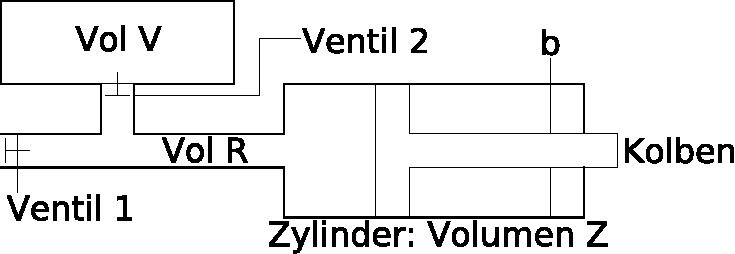
\includegraphics[width=0.8\textwidth]{include/evakuierungspumpe.pdf}
\begin{align*}
p_0: &\text{ Außendruck} \\
V: &\text{ zu evakuierendes Volumen} \\
R: &\text{ Restvolumen des Gestänges}
\end{align*}
\end{center}
%\end{minipage}

\begin{theorem}[Gasgesetz von Boyle-Mariotte]
\begin{align*}
p \cdot V = C \cdot m &&
\begin{aligned}
&p: \text{Druck} \\
&V: \text{Volumen} \\
&m: \text{Masse} \\
&C: \text{Boltzmann-Konstante}g
\end{aligned}
\end{align*}
\end{theorem}

\paragraph{Funktionsweise}
\begin{itemize}
  \item Kolben in Stellung b; Ventil 1 offen; Ventil 2 geschlossen; d.h. Außenluft
  \item Kolben fährt nach a; Ventil 2 geschlossen; Ventil 2 geschlossen
  \item Kolben fährt nach b; Ventil 1 geschlossen; Ventil 2 offen; d.h. evakuiert V
\end{itemize}
Ergebnis: schrittweise Änderung des Drucks

\paragraph{Modellierung}
\begin{enumerate}
	\item Kolbenhub (Stellung a)
	\begin{align*} \left.
		\begin{aligned}
			p_0 \cdot (V + R) &= C \cdot (m_v + m_r) \\
			\text{Kolben zu b} &= p_1 \cdot (V + R + Z)
		\end{aligned} \right\rangle
		p_1 = \frac{p_0 \cdot V + p_0 \cdot R}{V + R + Z}
	\end{align*}
	\item Kolbenschub
	\begin{align*}
	p_1 \cdot V + p_0 \cdot R &= p_2 \cdot (V + R + Z) && \text{Außendruck in R durch Öffnen des Ventils 1} \\
	p_2 &= \frac{p_1 \cdot V + p_0 \cdot R}{V + R + Z} \\
	&\vdots \\
	p_n &= \frac{p_{n-1} \cdot V + p_0 \cdot R}{V + R + Z} \\
	\end{align*}
\end{enumerate}
\begin{itemize} 
  \item Gibt es einen Grenzdruck $p_n \rightarrow p^*$?
  \item Auslegung von Z, R
\end{itemize}

\end{example}

\begin{definition}[Zahlenfolge]
Eine Funktion $f: \mathbb N \rightarrow \mathbb N$ heißt reelle (Zahlen)folge.\\
Notation: $f_n$ oder $(f_n)_{n \in \mathbb N}$
\end{definition}

\begin{example}
\begin{enumerate}
	\item $a_n = n$: $a_1 = 1, a_2 = 2, \ldots$
	
\begin{tikzpicture}
	[uplabel/.style={above=4mm,anchor=center},
	 downlabel/.style={below=4mm,anchor=center}]
%\draw (0.5,0) -- (3.5,0)
% LH: scaling
\draw (0.5,0) -- (5,0)
(1,0) node (a1) {} node[uplabel] {$a_1$} node[downlabel] {1}
(2.75,0) node (a2) {} node[uplabel] {$a_2$} node[downlabel] {2}
(4.5,0) node (a3) {} node[uplabel] {$a_3$} node[downlabel] {3};
\foreach \n in {a1,a2,a3}
\draw (\n) ++(0,-0.1) -- ++(0,0.2);
\end{tikzpicture}\hspace{1cm}
\begin{tikzpicture}[line cap=round,line join=round,>=triangle 45,x=1.0cm,y=1.0cm]
\draw[color=white] (-1,0) -- (-0.5,0);
\draw[->,color=black] (-0.5,0) -- (2.5,0);
\foreach \x in {,1,2}
\draw[shift={(\x,0)},color=black] (0pt,2pt) -- (0pt,-2pt) node[below] {\footnotesize $\x$};
\draw[->,color=black] (0,-0.5) -- (0,2.5);
\foreach \y in {,1,2}
\draw[shift={(0,\y)},color=black] (2pt,0pt) -- (-2pt,0pt) node[left] {\footnotesize $\y$};
\draw[color=black] (0pt,-10pt) node[right] {\footnotesize $0$};
\clip(-0.5,-0.5) rectangle (2.5,2.5);
\fill [color=black] (1,1) circle (1.5pt);
\fill [color=black] (2,2) circle (1.5pt);
\end{tikzpicture}

	\item $a_n = \frac{1}{n}$: $a_1 = 1, a_2 = \frac{1}{2}, a_3 = \frac{1}{3}, \ldots$\label{ex:nullfolge}
	
	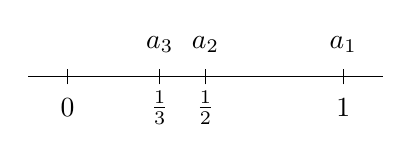
\begin{tikzpicture}
	[uplabel/.style={above=4mm,anchor=center},
	 downlabel/.style={below=4mm,anchor=center}]
% \draw (0.5,0) -- (3.5,0)
% LH: scaling
\draw (0.5,0) -- (5,0)
(1,0) node (n0) {}  node[downlabel] {0}
(4.5,0) node (a1) {} node[uplabel] {$a_1$} node[downlabel] {1}
(2.75,0) node (a2) {} node[uplabel] {$a_2$} node[downlabel] {$\frac{1}{2}$}
(2.17,0) node (a3) {} node[uplabel] {$a_3$} node[downlabel] {$\frac{1}{3}$};
\foreach \n in {n0, a1,a2,a3}
\draw (\n) ++(0,-0.1) -- ++(0,0.2);
\end{tikzpicture}\hspace{1cm}
\begin{tikzpicture}[line cap=round,line join=round,>=triangle 45,x=1.0cm,y=1.0cm]
\draw[color=white] (-1,0) -- (-0.5,0);
\draw[->,color=black] (-0.5,0) -- (3.5,0);
\foreach \x in {,1,2,3}
\draw[shift={(\x,0)},color=black] (0pt,2pt) -- (0pt,-2pt) node[below] {\footnotesize $\x$};
\draw[->,color=black] (0,-0.5) -- (0,1.5);
\foreach \y in {,1}
\draw[shift={(0,\y)},color=black] (2pt,0pt) -- (-2pt,0pt) node[left] {\footnotesize $\y$};
\draw[color=black] (0pt,-10pt) node[right] {\footnotesize $0$};
\clip(-0.5,-0.5) rectangle (3.5,1.5);
\fill [color=black] (1,1) circle (1.5pt);
\fill [color=black] (2,0.5) circle (1.5pt);
\fill [color=black] (3,0.33) circle (1.5pt);
\end{tikzpicture}

	\item $a_n = (-1)^n$: $a_1 = -1, a_2 = 1, \ldots$

	\begin{tikzpicture}
	[uplabel/.style={above=4mm,anchor=center},
	 downlabel/.style={below=4mm,anchor=center}]
%\draw (0.5,0) -- (3.5,0)
% LH: scaling
\draw (0.5,0) -- (5,0)
(2.75,0) node (n0) {}  node[downlabel] {0}
(1,0) node (a1) {} node[uplabel] {$a_1$}  node[downlabel] {-1}
(4.5,0) node (a2) {} node[uplabel] {$a_2$} node[downlabel] {1};
\foreach \n in {n0,a1,a2}
\draw (\n) ++(0,-0.1) -- ++(0,0.2);
\draw[color=white] (0,0) -- (0,-1.5);
\end{tikzpicture}\hspace{1cm}
\begin{tikzpicture}[line cap=round,line join=round,>=triangle 45,x=1.0cm,y=1.0cm]
\draw[color=white] (-1,0) -- (-0.5,0);
\draw[->,color=black] (-0.5,0) -- (4.5,0);
\foreach \x in {,1,2,3,4}
\draw[shift={(\x,0)},color=black] (0pt,2pt) -- (0pt,-2pt) node[below] {\footnotesize $\x$};
\draw[->,color=black] (0,-1.5) -- (0,1.5);
\foreach \y in {-1,1}
\draw[shift={(0,\y)},color=black] (2pt,0pt) -- (-2pt,0pt) node[left] {\footnotesize $\y$};
\draw[color=black] (0pt,-10pt) node[right] {\footnotesize $0$};
\clip(-0.5,-1.5) rectangle (4.5,1.5);
\fill [color=black] (1,-1) circle (1.5pt);
\fill [color=black] (2,1) circle (1.5pt);
\fill [color=black] (3,-1) circle (1.5pt);
\fill [color=black] (4,1) circle (1.5pt);
\end{tikzpicture}

\end{enumerate}
\end{example}

\paragraph{Frage}
Streben die Folgen gegen ausgezeichnete Werte?
Im Beispiel \ref{ex:nullfolge} ist es der Null-Wert: $a_n \rightarrow 0$.\\
Zentrale Werkzeuge: Schranken und Monotonie

\begin{definition}[Beschränktheit]
Eine reelle Folge $(a_n)_{n \in \mathbb N}$ heißt nach oben beschränkt, falls ein reelles $L$ existiert mit
\begin{equation*} a_n \le L\end{equation*}
analog: nach unten beschränkt
\begin{equation*} a_n \ge L\end{equation*}
\end{definition}

\begin{example}
\begin{enumerate}
	\item untere Schranke $1$, keine obere Schranke
	\item untere Schranke $0$, obere Schranke $1$
	\item untere Schranke $-1$, obere Schranke $1$
\end{enumerate}
\end{example}

\begin{example}[Evakuierungspumpe, Fortsetzung]
Druckfolge $p_n$
\begin{itemize}
\item nach unten durch 0 beschränkt (da nur positive Terme)
\item nach oben durch $p_0$ beschränkt
\begin{align*}
p_1 &= p_0 \cdot \frac{V + R}{V + R + Z} < p_0 \\
p_2 &= \frac{p_1 \cdot V + p_0 \cdot R}{V + R + Z} < \frac{p_0 \cdot V + p_0 \cdot R}{V + R + Z} < p_0 \\
p_n &\text{ analog}
\end{align*}
\end{itemize}
\end{example}

\begin{definition}[Monotonie]
Eine reelle Folge heißt monoton wachsend, wenn $\forall n \in \mathbb N : a_n \le a_{n+1}$ und
streng monoton wachsend, wenn $a_n < a_{n+1}$. Analog: (streng) monoton fallend.
\end{definition}
Anschaulich: monoton wachsend + obere Schranke $\Rightarrow$ Grenzwert existiert $\equiv$ Supremumaxiom $\mathbb R$